\clearpage

\section{공격 절차 라이브러리와 커버리지}\label{sec:abilities}

\subsection{Ability의 구성}\label{subsec:ability}

Ability는 모사할 공격 기법과 해당 기법의 실행 방법을 함께 정의한다.

\begin{itemize}
    \item \textbf{분류}: ATT\&CK 전술, 기법 ID(하위 기법 포함), 기법 이름을 정의하며, 관련 위협 그룹 및 CVE 정보를 추가할 수 있다.
    \item \textbf{실행 조건}: 대상 플랫폼과 명령 실행에 사용할 셸(실행기)을 지정하며, 실행기는 여러 개 등록할 수 있다.
    \item \textbf{명령}: 실제 실행할 명령문을 정의하며, 대상마다 달라지는 값은 \texttt{\#\{이름\}} 형태의 \textbf{변수}로 표시한다.
    \item \textbf{페이로드}: 명령 실행에 필요한 보조 파일의 목록을 정의한다(\ref{subsec:payload}절).
\end{itemize}

라이브러리는 공개된 공격 절차 자료를 수집·정리하여 구성하였다.
동일한 공격 절차라도 실행기·명령·페이로드의 조합이 다르면 각 변형을 별도의 Ability로 등록한다.
운영자는 화면에서 Ability를 검색·조회하고, 직접 작성한 절차를 추가할 수도 있다.

\paragraph{\textbf{실행기 선택:}}
동일한 Ability라도 에이전트마다 지원하는 셸이 다를 수 있다.
엔진은 Ability에 정의된 실행기를 순서대로 확인하여, 에이전트가 비컨을 통해 보고한 셸 목록과 일치하는 실행기 중 첫 번째 항목을 선택한다.
PowerShell 실행기는 두 가지 명칭으로 표기될 수 있으므로, 두 명칭을 동일한 실행기로 인식하도록 하였다.
에이전트가 지원하는 실행기가 없으면 해당 에이전트에서 단계를 실행하지 않고 상태를 `건너뜀'으로 기록한다.
이렇게 하면 Windows 전용 절차를 Linux 에이전트에서 실행하여 불필요한 오류가 발생하는 일을 방지하고, 해당 호스트에 적용되지 않는 단계임을 결과에 명확히 기록할 수 있다.

\subsection{ATT\&CK 커버리지}\label{subsec:coverage}

`ATT\&CK 커버리지' 화면은 공격 절차 라이브러리가 지원하는 기법의 범위를 ATT\&CK Enterprise 매트릭스를 기준으로 시각화한다(그림~\ref{fig:coverage}).
산정 방식은 다음과 같다.

\begin{itemize}
    \item 각 Ability의 기법 ID를 상위 기법 기준으로 집계한다. 하위 기법(예: T1059.004)을 실행하는 Ability는 상위 기법(T1059)을 지원하는 것으로 본다.
    \item 하나의 Ability에 여러 전술 또는 기법이 지정된 경우 각각을 별도로 집계한다.
    \item ATT\&CK 버전에 따라 명칭이나 구성이 달라진 전술(예: 방어 회피에서 갈라져 나온 은닉·방어 무력화)은 기준 매트릭스의 14개 전술에 맞춰 통합한다.
    \item 커버리지 산정 시 분모는 기준 매트릭스에 정의된 Enterprise 상위 기법의 전체 개수이며, 하나 이상의 Ability가 연결된 기법을 `지원 기법'으로 집계한다. 지원되지 않는 기법은 별도의 `미지원' 목록에서 확인할 수 있다.
    \item 기준 매트릭스는 2025년 12월 플랫폼에 등록된 ATT\&CK Enterprise 기법 목록이다.
\end{itemize}

매트릭스의 각 칸은 해당 기법에 대응하는 Ability 변형의 수에 따라 색상의 농도를 달리하며, Ability의 수가 많을수록 진한 색상으로 표시한다.

\begin{figure}[H]
\centering
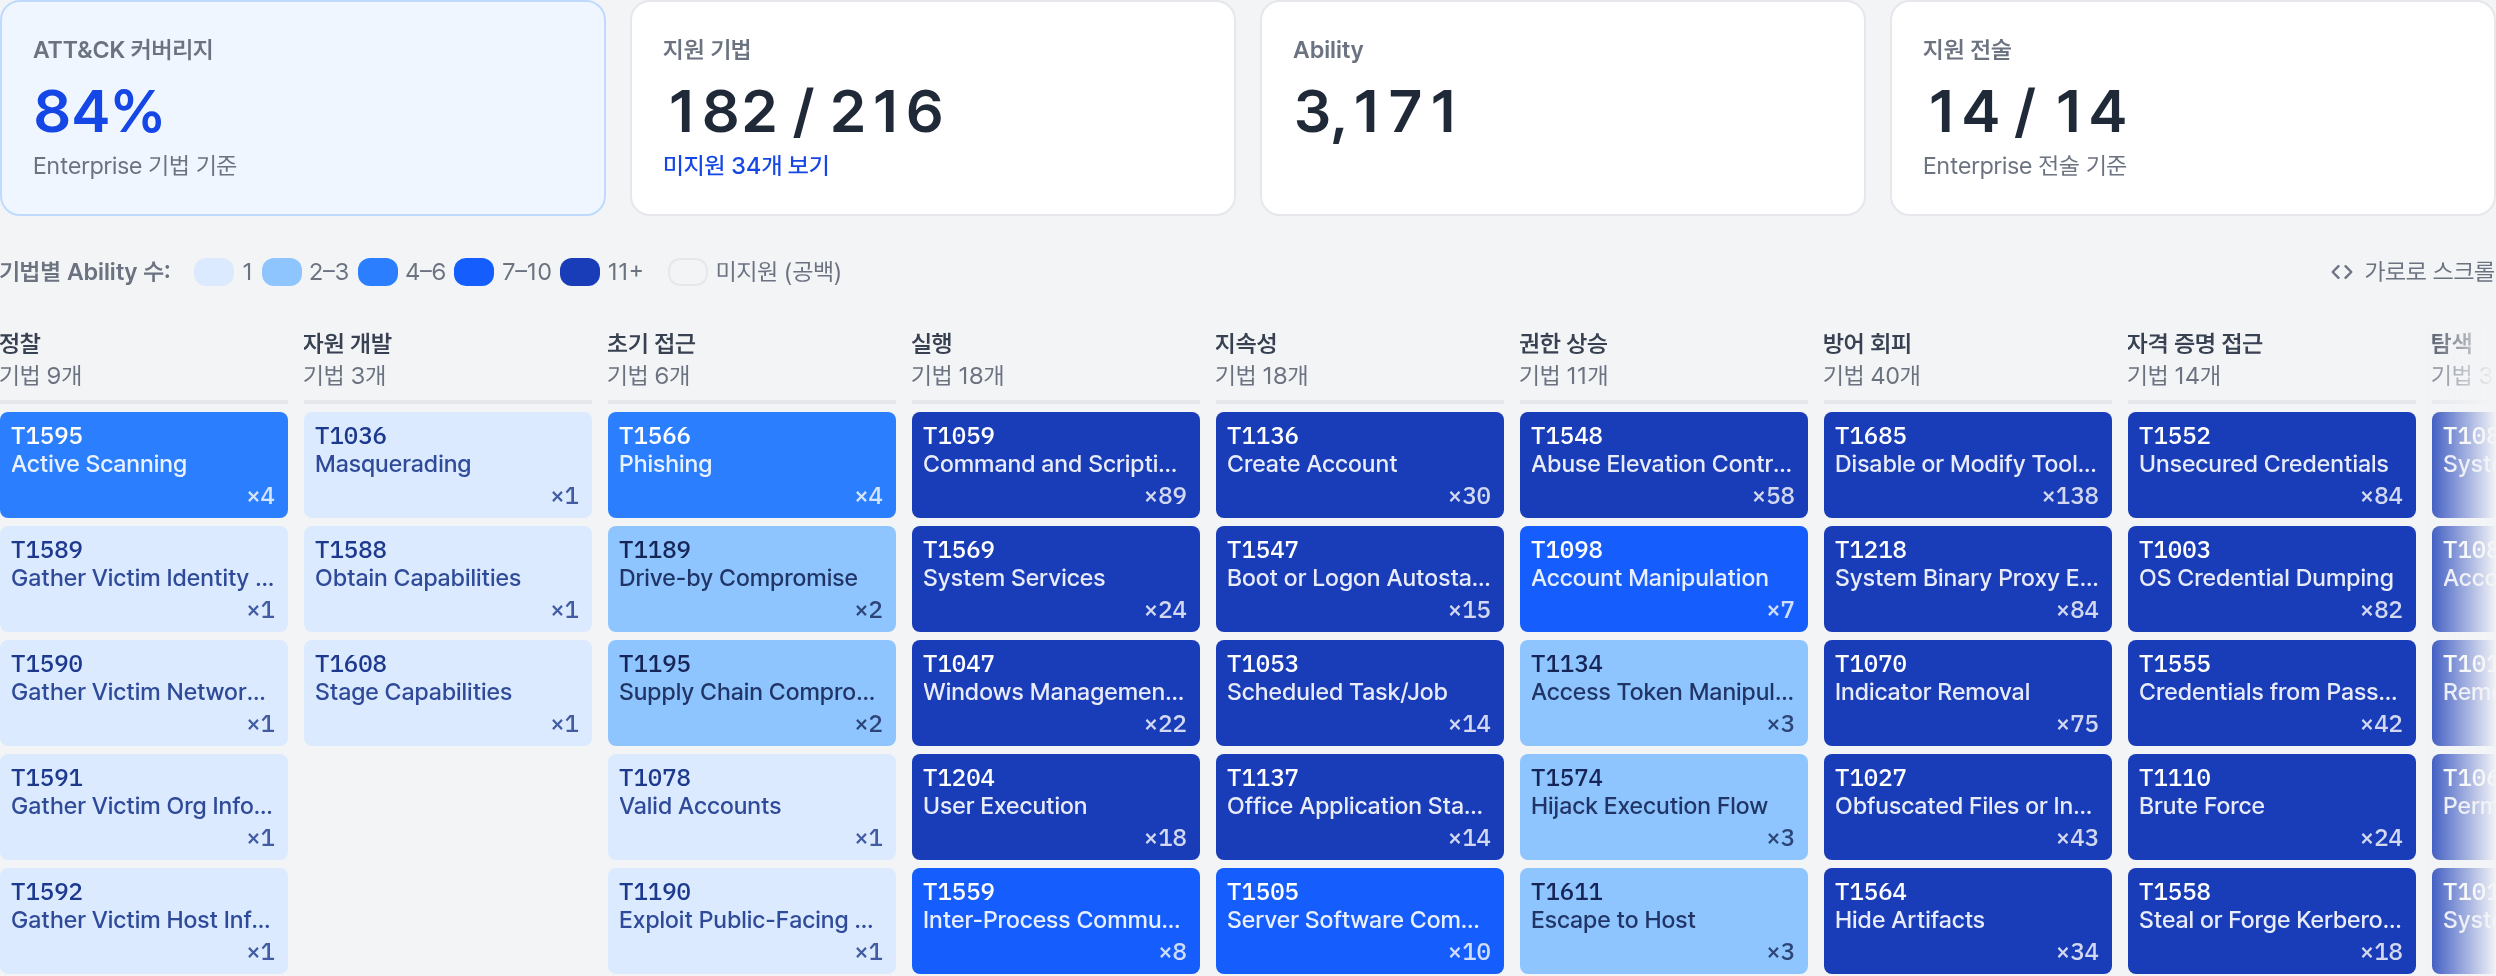
\includegraphics[width=\textwidth]{screenshots-bas/coverage.png}
\caption{ATT\&CK 커버리지 화면(요약 지표와 전술별 매트릭스 일부, 캡처 시점 기준)}
\label{fig:coverage}
\end{figure}

\paragraph{\textbf{해석상 주의:}}
커버리지 수치는 라이브러리의 Ability 추가·삭제 또는 기준 매트릭스 갱신에 따라 달라질 수 있다.
화면에 접근할 때마다 데이터베이스에 저장된 최신 정보를 기준으로 커버리지를 재산정하므로, 그림~\ref{fig:coverage}의 수치는 화면 캡처 시점의 산정 결과이다.
또한 이 수치는 라이브러리에 해당 기법을 실행할 수 있는 절차가 등록되어 있음을 의미할 뿐이다.
해당 절차가 특정 대상 환경에서 실제로 성공했는지, 방어 제품이 이를 탐지했는지, 해당 기법에 대한 시험이 실제로 수행되었는지는 보여 주지 않는다.
지원되는 공격 절차가 특정 플랫폼(예: Windows)에 편중되어 있는지도 이 화면만으로는 확인할 수 없다.
아울러 전술 분류가 명확하지 않아 ``복수 전술'' 등으로 지정된 Ability는 기법 수 산정에는 포함되지만, 14개 표준 전술 열에는 표시되지 않는다.
